\chapter{Experimental Setup}
\label{ch:setup}

\section{Robot Platform}

The experiments were conducted on \emph{Ricbot}, a compact wheeled sensor platform developed at DTU and used in the DTU robotic intercropping research project \cite{RoboticIntercroppingDTU2026}. Ricbot is designed for rapid field deployment: the chassis can be partially disassembled to fit within a $55\,\text{cm}$ vertical envelope so that it can be transported in a standard vehicle and carried by one or two people, with a total mass of approximately $25$--$30\,\text{kg}$ \cite{RicbotWiki}.

The drivetrain reuses the motors and wheels of the older \emph{Elektor Wheelie} platform, giving Ricbot a two-wheeled differential-drive configuration with passive support points. The on-board computer is a Raspberry Pi running ROS\,2, with a Teensy microcontroller handling low-level encoder and motor I/O. Sensor messages are bridged from MQTT into the ROS\,2 graph and synchronised across nodes via PTP (Precision Time Protocol). All sensor streams are written to timestamped plain-text log files on the on-board computer, one file per sensor per run.

%TODO: Maybe a better figure
\begin{figure}[H]
    \centering
    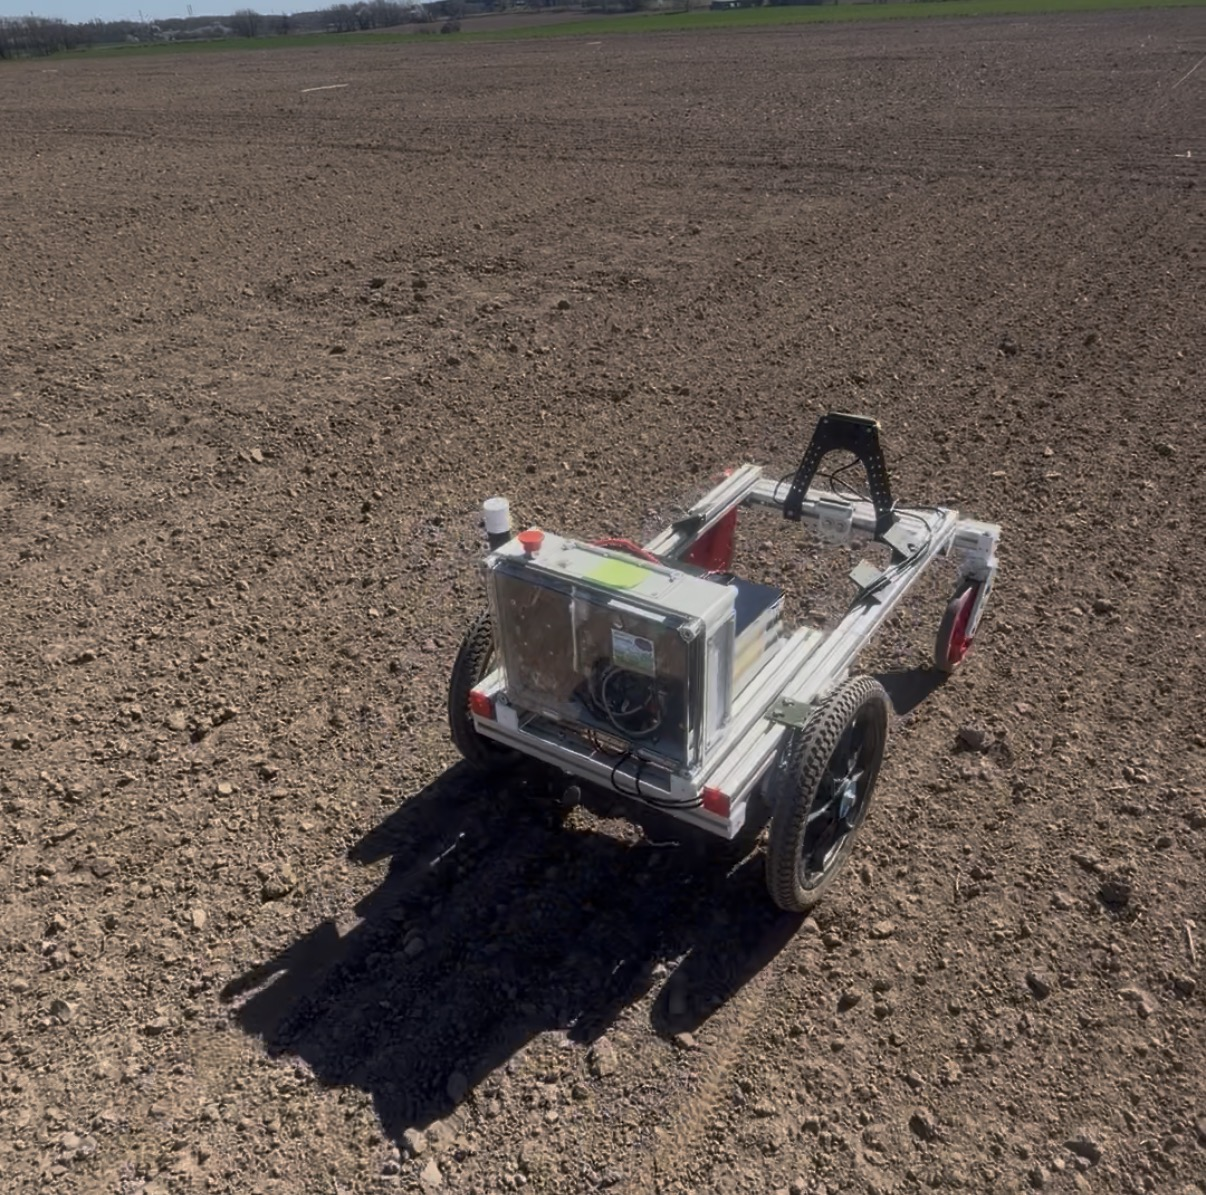
\includegraphics[width=0.5\textwidth]{Pictures/Photos/IMG_2983.jpg}
    \caption{The Ricbot platform used for data collection. Differential-drive chassis based on Elektor Wheelie hardware, with the on-board computer and IMU rigidly mounted to the central frame.}
    \label{fig:ricbot}
\end{figure}

\begin{figure}[H]
    \centering
    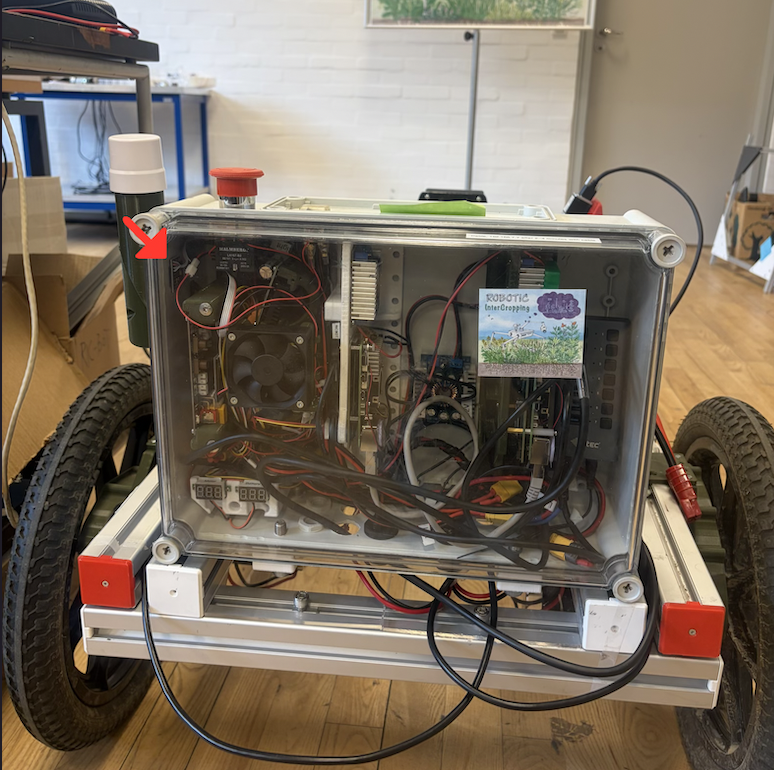
\includegraphics[width=0.5\textwidth]{Pictures/Photos/Screenshot 2026-05-13 at 18.06.50.png}
    \caption{Close-up of the IMU mounting location and wheel encoders, to show where the intrinsic sensors are physically attached to the chassis.}
    \label{fig:ricbot_back}
\end{figure}

%TODO: can add a more close up of the IMU


\section{Sensor Suite}

Three sensor modalities were used in this study; all are intrinsic to the robot and require no external infrastructure.

\subsection{Accelerometer and Gyroscope (IMU)}

A six-axis MEMS IMU of the InvenSense \texttt{MPU-9250} family, rigidly mounted to the robot chassis, provides linear accelerations and angular rates. The \texttt{MPU-9250} integrates a 3-axis accelerometer, a 3-axis gyroscope and a 3-axis magnetometer on a single die; only the accelerometer and gyroscope channels are used in this work, as the magnetometer is heavily disturbed by the robot's own motors and electronics. Accelerations are recorded in units of $g$ (so that the gravity axis reads approximately $-1\,g$ at rest) and angular rates in degrees per second. The IMU is driven from the Teensy~4.1 firmware via the \texttt{MPU9250\_asukiaaa} Arduino library, which initialises the accelerometer to a full-scale range of $\pm 4\,g$ (sensitivity $8192\,\text{LSB}/g$) and the gyroscope to $\pm 1000\,^{\circ}/\text{s}$ (sensitivity $32.8\,\text{LSB}/(^{\circ}/\text{s})$). The library does not write to the on-chip Digital Low-Pass Filter (DLPF) registers, so the sensor operates at its power-on defaults: an accelerometer bandwidth of $460\,\text{Hz}$ (internal sample rate $1\,\text{kHz}$) and a gyroscope bandwidth of $250\,\text{Hz}$ (internal sample rate $8\,\text{kHz}$). No firmware-level gyro bias correction is applied (\texttt{gyro\_offset = 0\,0\,0} in \texttt{robot.ini}). The Teensy forwards each new IMU reading to the Raspberry~Pi as it becomes available; across all production data-collection runs used in this thesis, the resulting log streams have a consistent median inter-sample interval of approximately $12\,\text{ms}$ ($\approx 83\,\text{Hz}$) for both the accelerometer and the gyroscope.
%A six-axis MEMS IMU of the InvenSense \texttt{MPU-9250} family, rigidly mounted to the robot chassis, provides linear accelerations and angular rates. The \texttt{MPU-9250} integrates a 3-axis accelerometer, a 3-axis gyroscope and a 3-axis magnetometer on a single die; only the accelerometer and gyroscope channels are used in this work, as the magnetometer is heavily disturbed by the robot's own motors and electronics. Accelerations are recorded in units of $g$ (so that the gravity axis reads approximately $-1\,g$ at rest) and angular rates in degrees per second. The IMU is driven from the Teensy~4.1 firmware via the \texttt{MPU9250\_asukiaaa} Arduino library, which initialises the accelerometer to a full-scale range of $\pm 4\,g$ (sensitivity $8192\,\text{LSB}/g$) and the gyroscope to $\pm 1000\,^{\circ}/\text{s}$ (sensitivity $32.8\,\text{LSB}/(^{\circ}/\text{s})$). The library does not write to the on-chip Digital Low-Pass Filter (DLPF) registers, so the sensor operates at its power-on defaults: an accelerometer bandwidth of $460\,\text{Hz}$ (internal sample rate $1\,\text{kHz}$) and a gyroscope bandwidth of $250\,\text{Hz}$ (internal sample rate $8\,\text{kHz}$). No firmware-level gyro bias correction is applied (\texttt{gyro\_offset~=~0\,0\,0} in \texttt{robot.ini}). The Teensy forwards each new IMU reading to the Raspberry~Pi as it becomes available; the resulting log streams have a median inter-sample interval of $12\,\text{ms}$ (approximately $83\,\text{Hz}$) for both the accelerometer and the gyroscope, with instantaneous rates varying between roughly $30$ and $130\,\text{Hz}$ due to firmware-loop jitter (characterised further in \Cref{ch:processing}).


The physical axis convention used throughout this thesis, verified empirically from rest-period accelerometer biases in the raw logs, is:
\begin{itemize}
    \item \textbf{Accelerometer:} $a_x$ — lateral (left/right), $a_y$ — vertical (gravity axis, $a_y \approx -1\,g$ at rest), $a_z$ — longitudinal (front/back).
    \item \textbf{Gyroscope:} $g_x$ — pitch rate, $g_z$ — roll rate. The yaw rate $g_y$ is \emph{excluded} from terrain features because it encodes intentional turning commands rather than terrain-induced motion.
\end{itemize}

Each accelerometer log line stores four whitespace-separated columns: the Unix timestamp in seconds and the three acceleration components $(a_x,a_y,a_z)$. Gyroscope logs follow the same convention for $(g_x,g_y,g_z)$. Comment lines at the top of each log file, prefixed with \texttt{\%}, describe the file type and column layout and are skipped during parsing (see \Cref{lst:acc_header}).

\begin{lstlisting}[language=, caption={Header of a raw accelerometer log.}, label={lst:acc_header}]
% Accelerometer logfile (IMU1)
% 1   Time (sec)
% 2-4 Accelerometer (x,y,z)
1771853111.8137  0.0624 -1.0024  0.0056
1771853111.8258  0.0562 -1.0027  0.0065
\end{lstlisting}

The tag \texttt{IMU1} indicates that the logging schema supports several IMUs in principle, although only one was active during this study.

\subsection{Wheel Odometry}

Wheel-encoder velocities are read by the Teensy microcontroller and forwarded to the Raspberry~Pi each time a new velocity estimate is available. The median inter-sample interval differs between collection campaigns: for the earlier Main runs (campus) the encoder stream is logged at approximately $130\,\text{Hz}$ (median interval $7.7\,\text{ms}$), whereas for the later Farm runs the rate was reduced to match the IMU at approximately $83\,\text{Hz}$ (median interval $12\,\text{ms}$). Each log line contains the timestamp, the left- and right-motor velocities $(v_1, v_2)$ in $\text{m}/\text{s}$, and two integer debug counters (encoder and velocity update numbers) which are discarded during preprocessing. A forward speed estimate is derived as the arithmetic mean of the two wheel speeds, $\bar v = (v_1 + v_2)/2$. All sensor streams are subsequently resampled onto a common $100\,\text{Hz}$ grid in preprocessing (\Cref{ch:processing}), so the per-campaign rate difference is absorbed before feature extraction. Wheel odometry contributes to features through speed-normalised statistics of the IMU signals and is used downstream to partition the feature table into two speed-regime sub-datasets (see \Cref{ch:feature}).

%\subsection{Pose Estimate}

%A pose stream is logged whenever a fused estimate is available. Each sample contains the timestamp, planar position $(x,y)$ in metres, heading $\theta$ in radians, and (when computed) a tilt angle in radians. Pose was used during labelling to verify route consistency between sessions, but it is \emph{not} used as a classification feature in any of the models evaluated in this thesis.

\section{Data Acquisition Setup}

All sensor streams are recorded simultaneously on the on-board Raspberry Pi during each run. A run begins when the robot is powered on and the logging service starts; it ends when logging is stopped manually. Each run therefore produces a single directory named \texttt{log\_YYYYMMDD\_HHMMSS.xxx}, where the suffix encodes the start time of the logger to millisecond resolution and the contained log files share a common run-relative timeline. A typical run directory layout is:

\begin{lstlisting}[language=, caption={Layout of one raw run directory.}]
log_20260421_113423.000/
|-- log_t0_acc_1.txt            % Accelerometer (IMU1)
|-- log_t0_gyro_1.txt           % Gyroscope     (IMU1)
|-- log_t0_encoder_velocity.txt % Odometry
|-- labels_config.json          % Terrain time ranges (post-hoc)
|-- metadata.md                 % Date, location, weather notes (post-hoc)
\end{lstlisting}

%|-- log_t0_pose.txt             % Only used for verification and not for 
%                                  analysis or classification
%Can add this if I decide to add the pose later on.

Time stamps in all logs are absolute Unix epoch seconds with sub-millisecond resolution, which allows the multi-sensor streams to be aligned to a common $100\,\text{Hz}$ grid in postprocessing (see \Cref{ch:processing}). Because each sensor is sampled by an independent firmware loop, the raw streams exhibit small per-sample jitter; this jitter is characterised in the sensor-quality-control reports produced for each run. The instantaneous sampling period was within $\pm 1\,\text{ms}$ of the median in 99\% of samples, and the worst-case observed period across all production runs was $29.2\,\text{ms}$ on the accelerometer (a $\sim$$2\times$ excursion from the nominal $12\,\text{ms}$). These rare gaps are detected and handled in the segmentation step (\Cref{ch:processing}).

No external sensors (camera, LiDAR, GNSS, motion capture) are used at any point in the pipeline, apart from post-hoc labeling of the classes. The decision to restrict the input to intrinsic sensors only is deliberate: it ensures that the resulting terrain classifier remains applicable in the visually degraded conditions for which exteroceptive sensing is unreliable (low light, dust, occlusion, or simply when no overhead infrastructure is available in a field deployment).










